\documentclass[12pt,a4paper,final,oneside]{book}
\usepackage[utf8]{inputenc}
\usepackage[portuguese]{babel}
\usepackage{cmbright}
%\usepackage[default]{frcursive}
\usepackage{yfonts}	
\usepackage{lettrine}
\usepackage{calligra}
\usepackage[T1]{fontenc}
\usepackage{amsmath}
\usepackage{amsfonts}
\usepackage{amssymb}
\usepackage{makeidx}
\usepackage{graphicx}
\usepackage{hyperref}
\usepackage{siunitx}
\usepackage{lipsum}  
\usepackage[alf]{abntex2cite}
\usepackage[left=2cm,right=2cm,top=2cm,bottom=2cm]{geometry}


\renewcommand{\LettrineFontHook}{\calligra}

%\renewcommand{\familydefault}{\sfdefault}
%\renewcommand{\ttdefault}{bch}


\begin{document}

\frontmatter
\begin{titlepage}
	\centering
	
\includegraphics[width=0.15\textwidth]{furg.eps}\par\vspace{1cm}
	{\scshape\LARGE Universidade Federal do Rio Grande - FURG \par}
	\vspace{0.5cm}
	{\scshape\Large  Centro de Ciências Computacionais\par}
		\vspace{5cm}
	{\scshape\LARGE Memorial Descritivo\par}
	%\vspace{1.5cm}
	%{\bfseries Progressão para professor Titular\par}
	\vspace{2cm}
	{\Large\itshape Nome Sobrenome Autor\par}
	\vfill
	{\large \today\par}
\end{titlepage}


\newenvironment{acknowledgements}%
    {\cleardoublepage\thispagestyle{empty}\null\vfill}%
    {\vfill\null}
        \begin{acknowledgements}
       Memorial Descritivo apresentado à Comissão Examinadora da Universidade Federal
do Rio Grande - FURG como parte dos requisitos para progressão funcional para a
Classe E do Magistério Superior (Professor Titular).
        \end{acknowledgements}
        



\chapter{Dedicatória}

\begin{itemize}
\item \lipsum [1]
\item \lipsum [2]
\item \lipsum [3]


\end{itemize}

\chapter{Agradecimentos}

\begin{itemize}

\item \lipsum [4]
\item \lipsum [5]
\item \lipsum [6]


\end{itemize}

\cleardoublepage

\tableofcontents

\listoffigures

\mainmatter

\chapter{Identificação}

\lettrine[lines=2, lhang=0.33, loversize=0.25, findent=1.5em]{A}{qui} começa o parágrafo
\lipsum[7]. 

\begin{itemize}
\item \textbf{CI}: xxxxxxxxxxx
\item \textbf{CPF}: xxxxxxxxxxx
\item \textbf{Matrícula SIAPE}: xxxxxxxxxxx
\item \textbf{Endereço Profissional}: Universidade Federal do Rio Grande, Centro de Ciências Computacionais - C3, Av Itália km 8 s/n - Caixa Postal 474 CEP 96200-970 Rio Grande, RS, BRASIL
\item \textbf{E-mail}: \url{xxxxxxxxxxx@gmail.com}, \url{xxxxxxxxxxx@furg.br}
\item \textbf{CV Lattes}: \url{http://lattes.cnpq.br/xxxxxxxxxxx}
\item \textbf{Cargo atual}: Professor Associado D/704


\end{itemize}



% este é um capítulo opcional, porém eu considero importante para construir o caminho
% para a atuação profissional docente na FURG.
\chapter{Pré-FURG}

\lettrine[lines=2, lhang=0.33, loversize=0.25, findent=1.5em]{N}{este} capítulo \lipsum[8].


\section{Infância}

\lipsum[10]

\lipsum[11]

\lipsum[12]


\begin{figure}
	\centering
		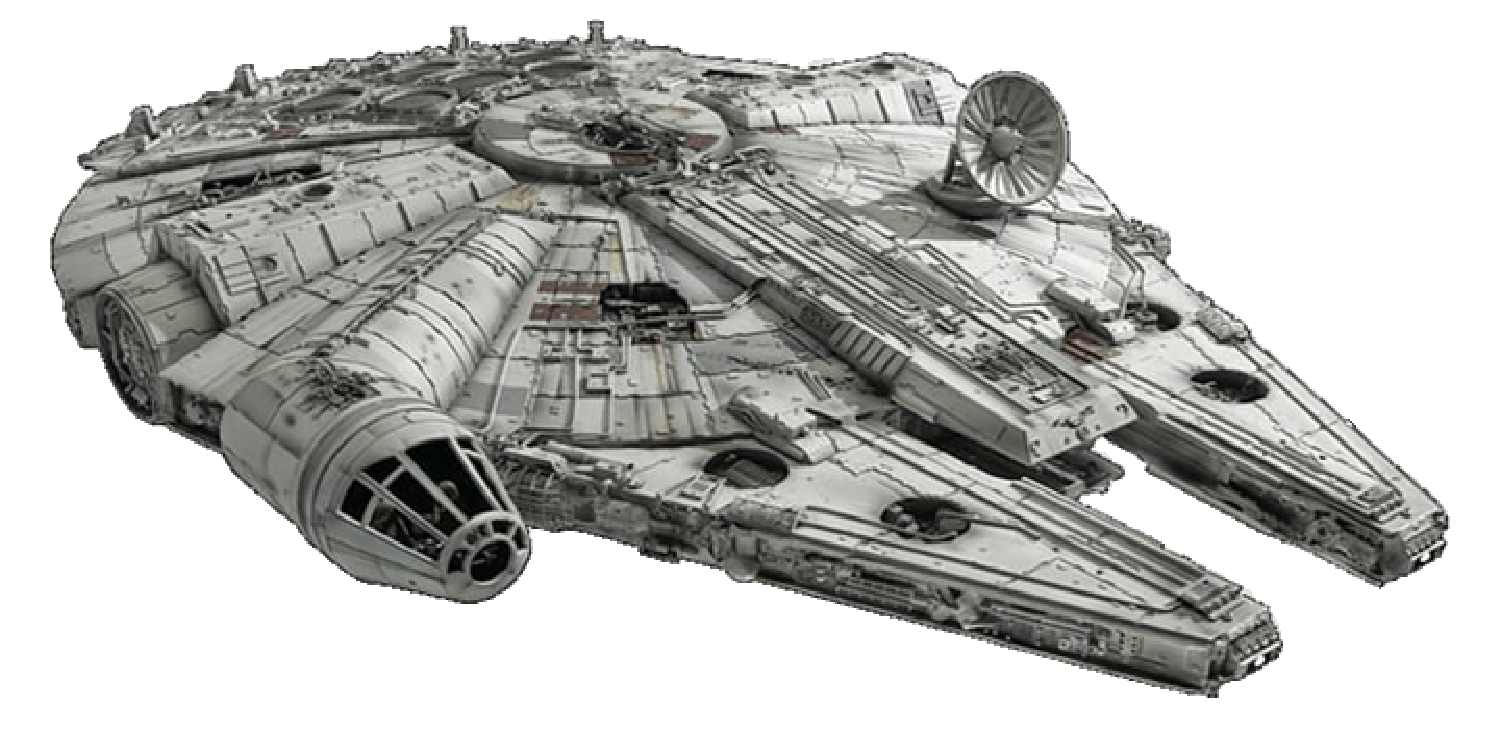
\includegraphics[width=0.99\textwidth,angle=-0]{Figuras/starwars_1.pdf}
		\caption[Linha do tempo pré FURG]{{\footnotesize Exemplo de figura.}}
		\label{fig:gantt}
\end{figure}

\section{Ensino Médio}
\lipsum[13] 

\lipsum[14]

\lipsum[15]

\lipsum[16]



\section{Graduação}

\lipsum[17]

\lipsum[18]

\lipsum[19]

\chapter{Formação Acadêmica}

%Descreva sua trajetória acadêmica, destacando suas conquistas, como diplomas, certificações e pós-graduações.
%
%Enfatize a relevância da sua formação para a área de atuação em que está buscando a promoção.
	
\lettrine[lines=2, lhang=0.33, loversize=0.25, findent=1.5em]{M}{ inha} \lipsum[17]


\section{Mestrado}
\lipsum[18]

\lipsum[19]

\lipsum[20]

\lipsum[21]

\lipsum[22]



\section{Doutorado}

\lipsum[23]

\lipsum[24]

\lipsum[25]

\lipsum[26]

\lipsum[27]

\begin{figure}
	\centering
		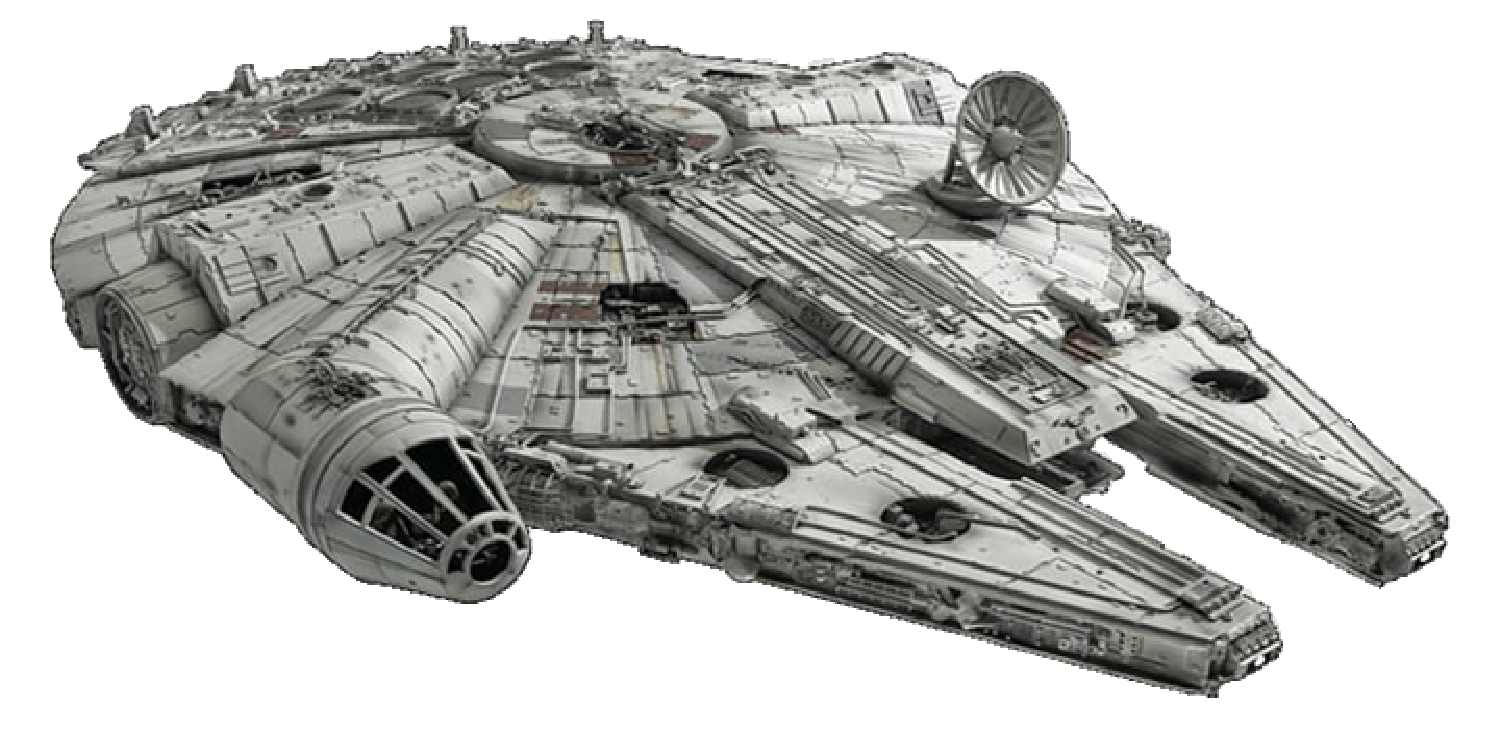
\includegraphics[width=0.99\textwidth,angle=-0]{Figuras/starwars_1.pdf}
		\caption[Linha do tempo pré FURG]{{\footnotesize Exemplo de figura.}}
		\label{fig:gantt2}
\end{figure}


\lipsum[28]

\lipsum[29]

\lipsum[30]

\lipsum[31]

\lipsum[32]

\section{Pós doutorado}

\lipsum[33]

\lipsum[34]








\chapter{O começo da carreira docente na FURG}

\lettrine[lines=2, lhang=0.33, loversize=0.25, findent=1.5em]{E}{ ste} capítulo
\lipsum[40]. 


\section{A Universidade Federal do Rio Grande - FURG}

\lipsum[41]
\cite{fake1}
\cite{fake2}

\lipsum[42]

\lipsum[43]

\lipsum[44]

\lipsum[45]


\section{O Centro de Ciências Computacionais}
\lipsum[46]

\lipsum[47]

\lipsum[48]



\section{Concurso e início na FURG}

\lipsum[49]

\lipsum[50]

\lipsum[51]




\chapter{Atividades de Administração Acadêmicas}

%Caso tenha exercido funções administrativas, como coordenação de curso, participação em comissões ou conselhos, descreva essas experiências.
%
%Resalte como essas atividades contribuíram para o crescimento e desenvolvimento da instituição.

\lettrine[lines=2, lhang=0.33, loversize=0.25, findent=1.5em]{A}{presento} 
\lipsum[50]


\section{Atividade a}
\lipsum[49]

\lipsum[50]

\lipsum[51]

\section{Atividade b}
\lipsum[52]

\lipsum[53]

\lipsum[54]

\section{Atividade c}

\lipsum[55]

\lipsum[56]

\lipsum[57]


\chapter{Atividades de Ensino}


% Aborde suas atividades de ensino, incluindo disciplinas lecionadas, metodologias inovadoras, orientações de alunos de graduação e pós-graduação.
% 
%  Destaque feedbacks positivos de alunos e resultados de pesquisas sobre a eficácia de suas práticas pedagógicas.

\lettrine[lines=2, lhang=0.33, loversize=0.25, findent=1.5em]{A}{presento} 
\lipsum[50]


\section{Atividade a}
\lipsum[60]

\lipsum[61]

\lipsum[62]

\section{Atividade b}
\lipsum[63]

\lipsum[65]

\lipsum[66]

\section{Atividade c}

\lipsum[64]

\lipsum[67]

\lipsum[68]

\chapter{Atividades de Pesquisa}


%Apresente suas contribuições significativas para a pesquisa na sua área.
%
%Destaque publicações em periódicos renomados, participação em conferências, projetos de pesquisa liderados e colaborações acadêmicas.

\lettrine[lines=2, lhang=0.33, loversize=0.25, findent=1.5em]{A}{presento} 
\lipsum[50]


\section{Atividade a}
\lipsum[49]

\lipsum[50]

\lipsum[51]

\section{Atividade b}
\lipsum[52]

\lipsum[53]

\lipsum[54]

\section{Atividade c}

\lipsum[55]

\lipsum[56]

\lipsum[57]




\chapter{Atividades de Extensão}


% Demonstre seu envolvimento em atividades de extensão, projetos com impacto na comunidade e serviços prestados à sociedade.
%Destaque eventos, palestras, consultorias ou projetos em que você desempenhou um papel ativo fora do ambiente acadêmico.


\lettrine[lines=2, lhang=0.33, loversize=0.25, findent=1.5em]{A}{presento} 
\lipsum[50]


\section{Atividade a}
\lipsum[49]

\lipsum[50]

\lipsum[51]

\section{Atividade b}
\lipsum[52]

\lipsum[53]

\lipsum[54]

\section{Atividade c}

\lipsum[55]

\lipsum[56]

\lipsum[57]

\chapter{Colaborações e Redes de Pesquisa}

%Destaque suas colaborações com outros pesquisadores e participação em redes de pesquisa.
%
%Mostre como essas parcerias contribuíram para o avanço do conhecimento em sua área.


\lettrine[lines=2, lhang=0.33, loversize=0.25, findent=1.5em]{A}{presento} 
\lipsum[50]


\section{Atividade a}
\lipsum[49]

\lipsum[50]

\lipsum[51]

\section{Atividade b}
\lipsum[52]

\lipsum[53]

\lipsum[54]

\section{Atividade c}

\lipsum[55]

\lipsum[56]

\lipsum[57]



\chapter{Projetos Futuros}

%Destaque suas colaborações com outros pesquisadores e participação em redes de pesquisa.
%
%Mostre como essas parcerias contribuíram para o avanço do conhecimento em sua área.


\lettrine[lines=2, lhang=0.33, loversize=0.25, findent=1.5em]{A}{presento} 
\lipsum[110]

\lipsum[49]

\lipsum[50]

\lipsum[51]


\chapter{Conclusão}

%
%Faça uma conclusão que reforce sua qualificação para a promoção.
%
%Destaque sua visão para o futuro, indicando como pretende contribuir para a instituição como professor titular.

\lettrine[lines=2, lhang=0.33, loversize=0.25, findent=1.5em]{A}{presento} 
\lipsum[75]

\lipsum[76]

\lipsum[77]



%




%**Dicas Gerais:**
%   - Mantenha uma linguagem clara e objetiva.
%   - Utilize evidências quantitativas sempre que possível (número de publicações, índice H, avaliações positivas, etc.).
%   - Seja honesto sobre desafios enfrentados, destacando como você os superou.
%
%Lembre-se de personalizar o memorial de acordo com suas experiências específicas e os critérios de promoção da sua instituição. 


\appendix
\chapter{Diplomas}
\section{Curso Técnico}
\label{app:dipl}


\section{Graduação}



\section{Mestrado}



\section{Doutorado}


\section{Revalidação de Doutorado}


\chapter{Atas e Portarias}

%\chapter{Diploma de Técnico em Instrumentação}
%\label{app:diplTec}
%\begin{figure}[h]
%	\centering
%		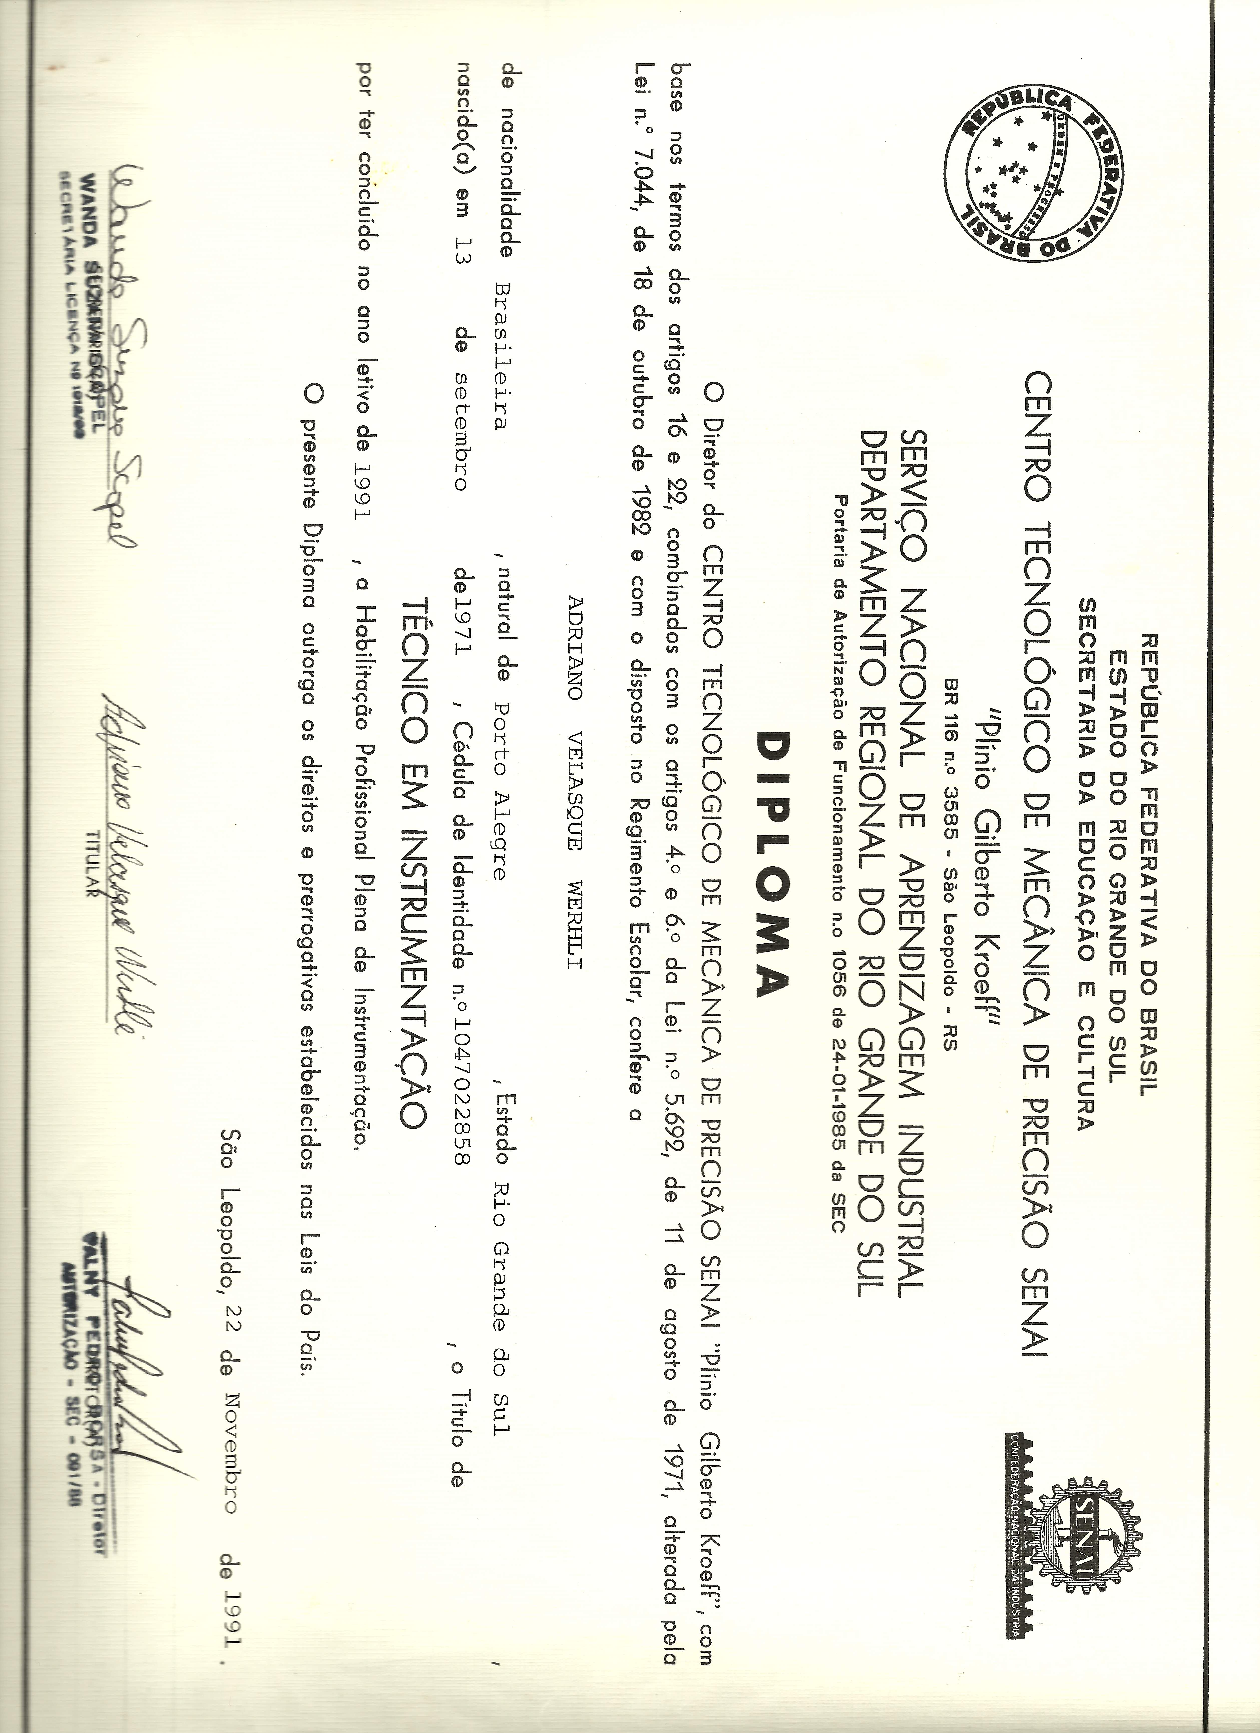
\includegraphics[width=0.7\textwidth,angle=90]{Figuras/diplTecInst.pdf}
%		\caption[Diploma de Técnico em Instrumentação]{Diploma do curso Técnico em Instrumentação do Senai, Cetemp, São Leopoldo - RS}
%		\label{fig:diplTec}
%\end{figure}
%
%
%\chapter{Diploma de Graduação}
%\label{app:diplGrad}
%\begin{figure}[h]
%	\centering
%		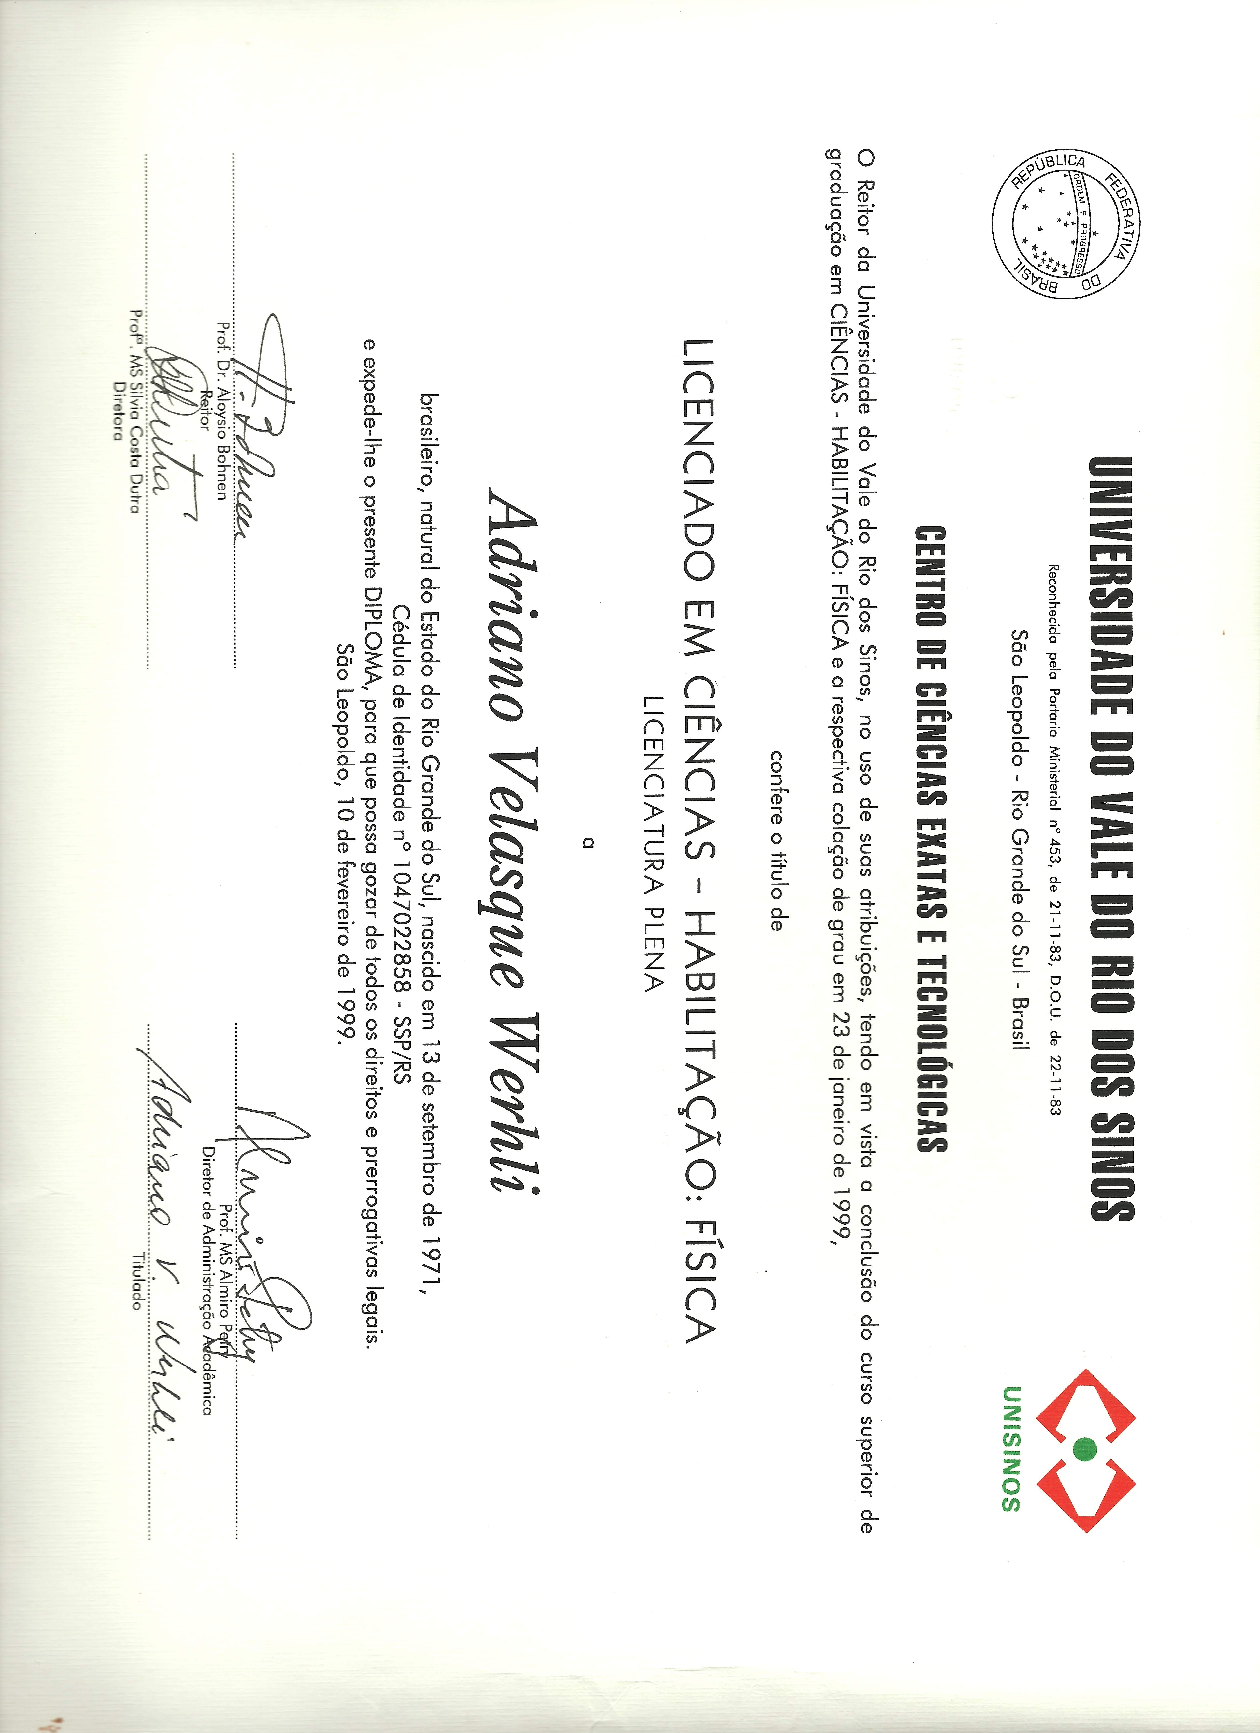
\includegraphics[width=0.7\textwidth,angle=90]{Figuras/diplFisica.pdf}
%		\caption[Diploma de Graduação em Física]{Diploma de Graduação em Licenciatura em Física, São Leopoldo - RS}
%		\label{fig:diplGrad}
%\end{figure}
%
%\chapter{Diploma de Mestrado}
%\label{app:diplMest}
%\begin{figure}[h]
%	\centering
%		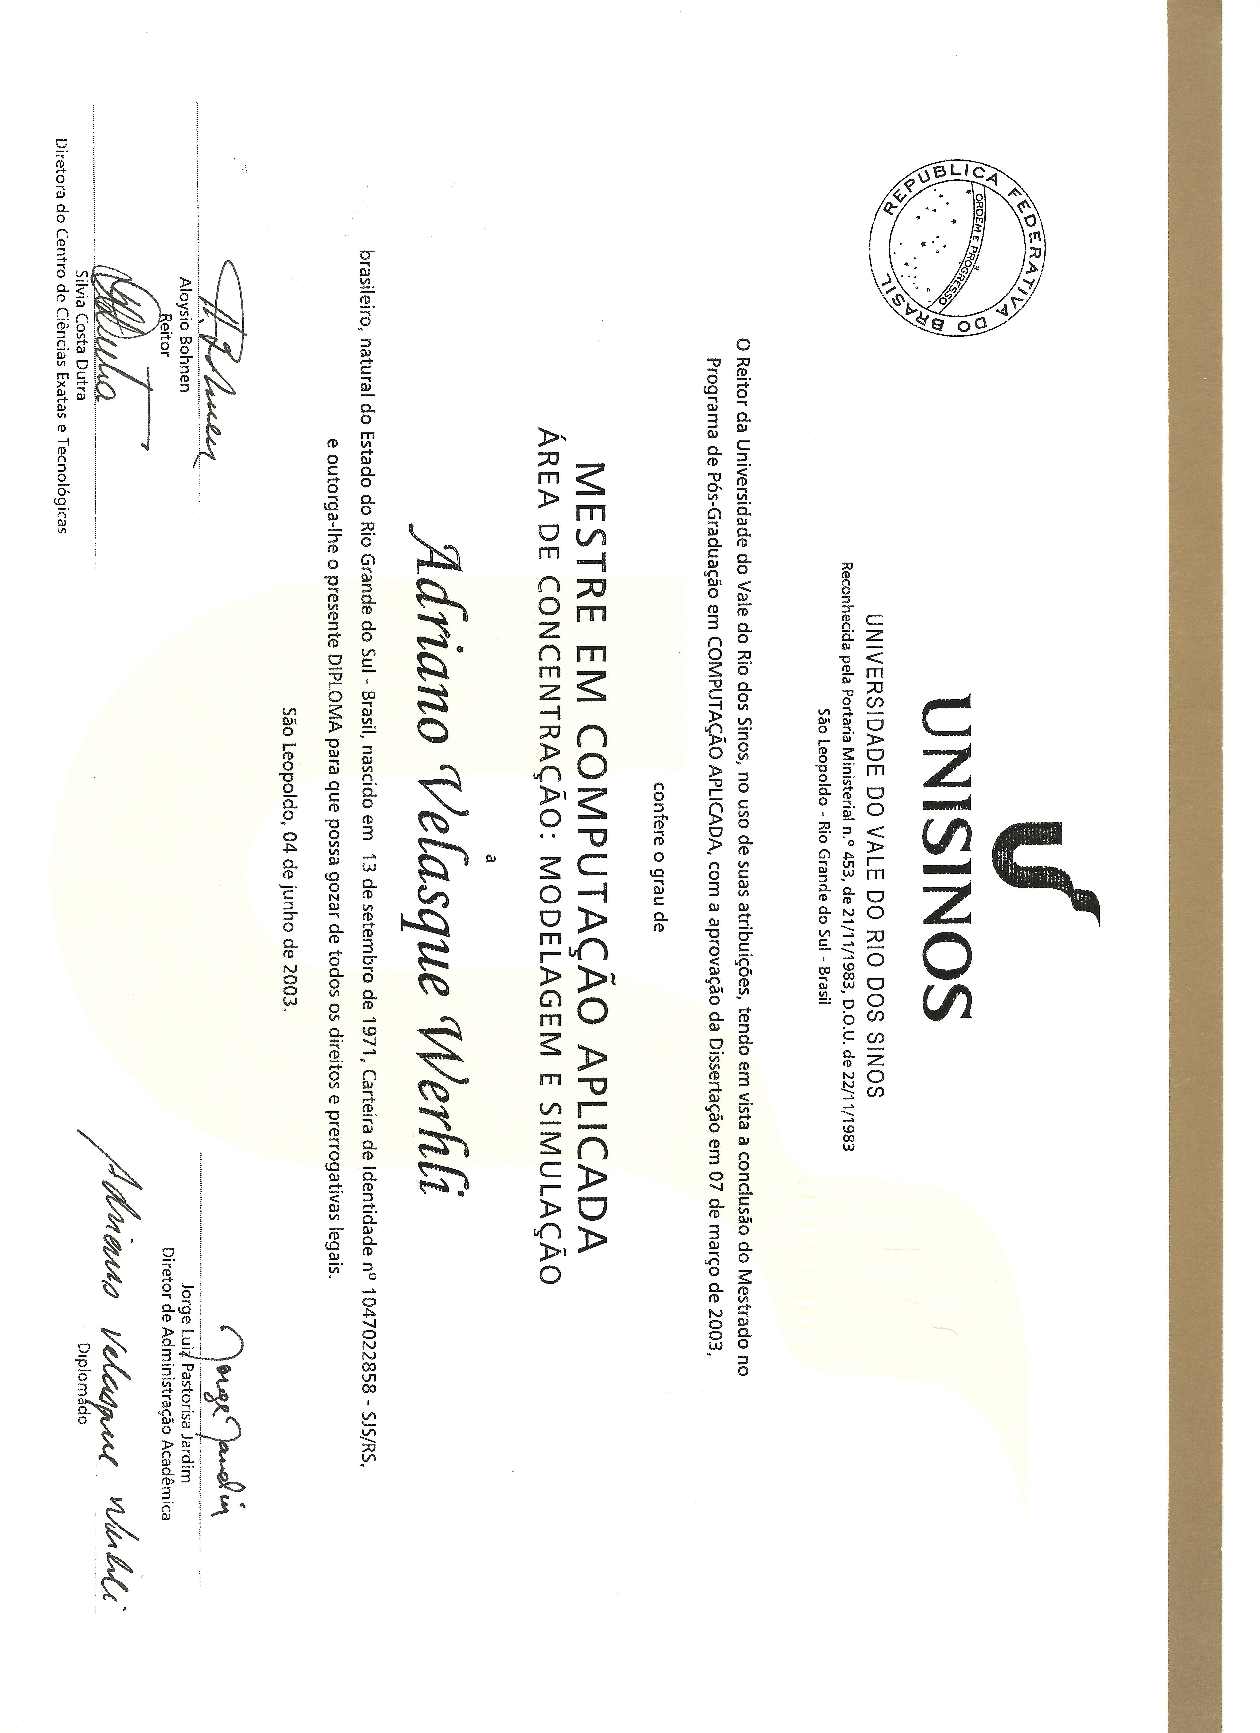
\includegraphics[width=0.7\textwidth,angle=90]{Figuras/diplMest.pdf}
%		\caption[Diploma de Mestrado em Computação Aplicada]{Diploma do Curso de Mestrado em Computação Aplicada, São Leopoldo - RS}
%		\label{fig:diplMest}
%\end{figure}
%
%
%\chapter{Diploma de Doutorado}
%\label{app:diplPhD}
%\begin{figure}[h]
%	\centering
%		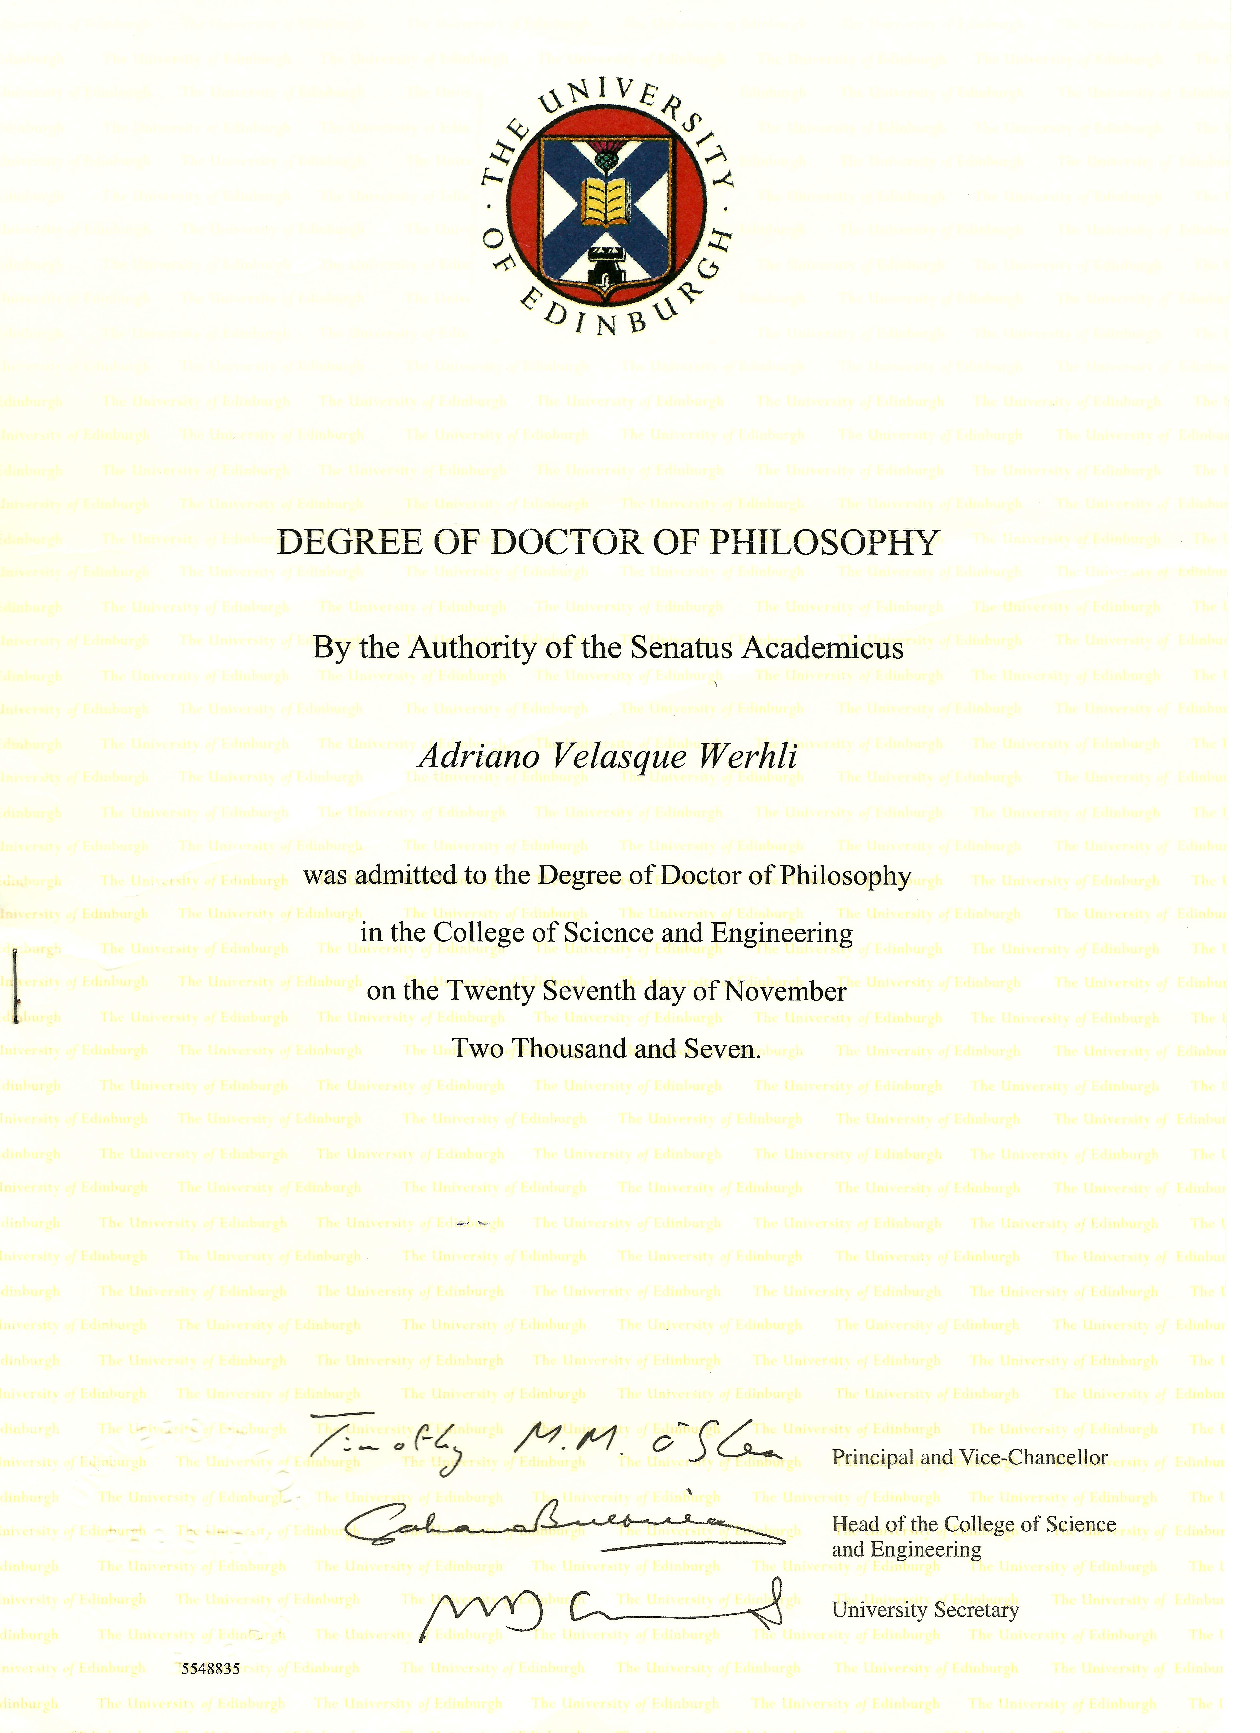
\includegraphics[width=0.7\textwidth,angle=0]{Figuras/diplPhD.pdf}
%		\caption[Diploma de Doutorado em Computação]{Diploma do Curso de Doutorado em Computação, Edinburgh, UK}
%		\label{fig:diplPhD}
%\end{figure}
%
%\chapter{Validação do Diploma de Doutorado}
%\label{app:diplPhDApostila}
%\begin{figure}[h]
%	\centering
%		\includegraphics[width=0.7\textwidth,angle=0]{Figuras/diplPhDApostila.pdf}
%		\caption[Revalidação do Diploma de Doutorado em Computação]{Revalidação do Diploma do Curso de Doutorado em Computação, Edinburgh, UK}
%		\label{fig:diplPhDApostila}
%\end{figure}


\bibliographystyle{abntex2-alf}
\bibliography{fake}

\end{document}